
\subsection*{A.1~偽代碼}
\begin{algorithm} 
	\SetAlgoVlined %设置带水平线的连线
	\caption{identifyRowContext} 
	\KwIn{$r_i$, $Backgrd(T_i)$=${T_1,T_2,\ldots ,T_n}$ and similarity threshold $\theta_r$} 
	\KwOut{$con(r_i)$} 
	$con(r_i)= \Phi$\; 
	\For{$j=1;j \le n;j \ne i$} 
	{ 
		float $maxSim=0$\; 
		$r^{maxSim}=null$\; 
		\While{not end of $T_j$} 
		{ 
			compute Jaro($r_i,r_m$)($r_m\in T_j$)\; 
			\If{$(Jaro(r_i,r_m) \ge \theta_r)\wedge (Jaro(r_i,r_m)\ge r^{maxSim})$} 
			{ 
				replace $r^{maxSim}$ with $r_m$\; 
			} 
		} 
		$con(r_i)=con(r_i)\cup {r^{maxSim}}$\; 
	} 
	return $con(r_i)$\; 
\end{algorithm}


\subsection*{A.2~smithchart mirrored}
\begin{figure}[H]
	\centering
	\begin{tikzpicture}[scale=1.2]
	\begin{smithchart}[smithchart mirrored,]
	\addplot coordinates {
		(0.5,0.2) (1,0.8) (2,2)
	};
	\end{smithchart}
	\end{tikzpicture}
	
\end{figure}














\subsection*{A.3~plot3D}
\begin{figure}[H]

	\begin{subfigure}{.49\textwidth}
		\centering
		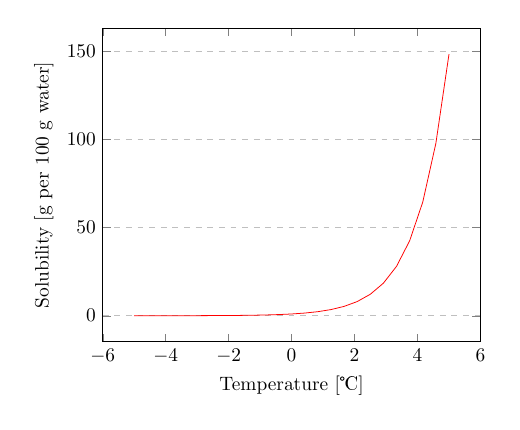
\begin{tikzpicture}[scale=0.7]
		\begin{axis}[
		xlabel={Temperature [\textcelsius]},
		ylabel={Solubility [g per 100 g water]},
		ymajorgrids=true,
		grid style=dashed,]
		\addplot[color=red]{exp(x)};
		\end{axis}
		\end{tikzpicture}
		\caption{A subfigure}
	\end{subfigure}
%-----------------------------------------------------------
	\begin{subfigure}{.49\textwidth}
		\centering
		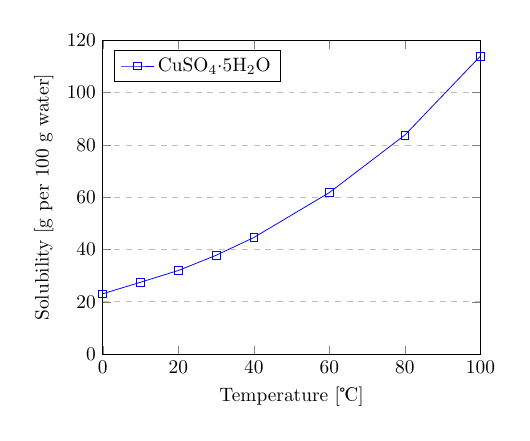
\begin{tikzpicture}[scale=.7]
			\begin{axis}[
				xlabel={Temperature [\textcelsius]},
				ylabel={Solubility [g per 100 g water]},
				xmin=0, xmax=100,
				ymin=0, ymax=120,
				xtick={0,20,40,60,80,100},
				ytick={0,20,40,60,80,100,120},
				legend pos=north west,
				ymajorgrids=true,
				grid style=dashed,
				]
				\addplot[
				color=blue,
				mark=square,
				]
				coordinates {
					(0,23.1)(10,27.5)(20,32)(30,37.8)(40,44.6)(60,61.8)(80,83.8)(100,114)
				};
				\legend{CuSO$_4\cdot$5H$_2$O}
			\end{axis}
		\end{tikzpicture}
		\caption{A subfigure}
	\end{subfigure}
%-----------------------------------------------------------
	\centering
	\begin{subfigure}{.49\textwidth}
		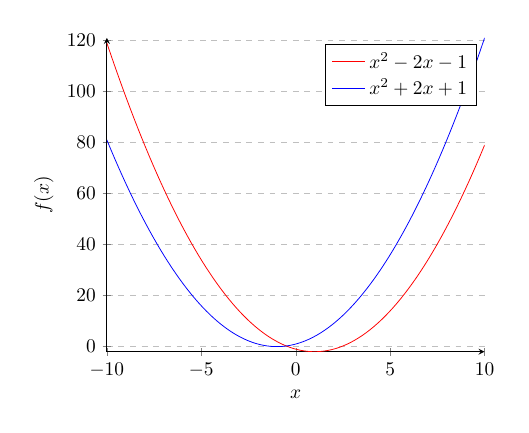
\begin{tikzpicture}[scale=0.7]
			\begin{axis}[
				axis lines = left,
				xlabel = $x$,
				ylabel = {$f(x)$},
				ymajorgrids=true,
				grid style=dashed,]
				]
				%Below the red parabola is defined
				\addplot [
				domain=-10:10, 
				samples=100, 
				color=red,
				]
				{x^2 - 2*x - 1};
				\addlegendentry{$x^2 - 2x - 1$}
				%Here the blue parabloa is defined
				\addplot [
				domain=-10:10, 
				samples=100, 
				color=blue,
				]
				{x^2 + 2*x + 1};
				\addlegendentry{$x^2 + 2x + 1$}
			\end{axis}
		\end{tikzpicture}
		\caption{A subfigure}
	\end{subfigure}
\end{figure}




\subsection*{A.4~plot3D}
\begin{figure}[H]
	\centering
	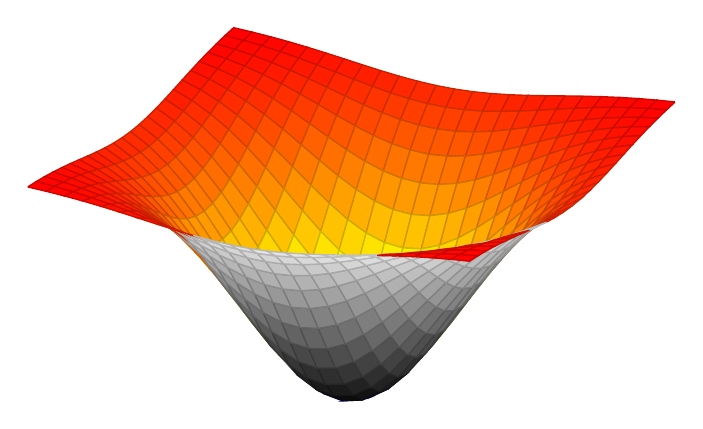
\begin{tikzpicture}[scale=1.2]
	\begin{axis}[
	hide axis,
	xlabel=$x$,ylabel=$y$,
	mesh/interior colormap name=hot,
	colormap/blackwhite,
	]
	\addplot3 [domain=-1.5:1.5,surf]
	{-exp(-x^2-y^2)};
	\end{axis}
	\end{tikzpicture}

app:plot3D
\end{figure}